\documentclass{revtex4-2}
\usepackage{siunitx}
\usepackage{graphicx}

\begin{document}

\title{Healing Gradient Degradation in Nb\textsubscript{3}Sn SRF Cavities Using a Recoating Method}
\author{Eric Viklund}
\email{ericviklund2023@u.northwestern.edu}
\affiliation{Department of Materials Science and Engineering, Northwestern University}
\affiliation{Fermi National Accelerator Laboratory}
\author{David N. Seidman}
\affiliation{Department of Materials Science and Engineering, Northwestern University}
\author{Sam Posen}
\email{sposen@fnal.gov}
\affiliation{Fermi National Accelerator Laboratory}
\author{Brad M. Tennis}
\affiliation{Fermi National Accelerator Laboratory}


\date{\today}

\begin{abstract}

    Despite having advantageous superconducting properties, Nb\textsubscript{3}Sn SRF cavities still have practical challenges compared to Nb SRF cavities due to the brittle nature of Nb\textsubscript{3}Sn. Performance degradation can occur when a Nb\textsubscript{3}Sn experiences mechanical stresses such as during handling and tuning of the cavity. In this study, we present a potential treatment for cavities that have experienced stress induced performance degradation that involves a recoating procedure. The degraded cavity is coated with a small amount of Sn using a single step vapor-diffusion method. Using this procedure we are able to recover a significant portion of the lost performance of a Nb\textsubscript{3}Sn SRF cavity.

\end{abstract}

\maketitle

\section{Introduction}
\label{sec:Introduction}

Niobium cavities have been extensively studied and treatments have been developed to optimize the accelerating gradient and quality factor~\cite{10.1063/1.4866013, 10.1063/1.4960801, 10.1063/5.0059464, 10.1063/5.0063379}. However, the performance of niobium SRF cavities is still limited by the material properties of niobium. A promising alternative to niobium is Nb\textsubscript{3}Sn. For several decades researchers have been working to implement Nb\textsubscript{3}Sn in superconducting radiofrequency (SRF) cavities.\cite{10.1063/1.4913617, 10.1063/1.4913247} Desirable superconducting properties, such as higher superconducting transition temperature (T\textsubscript{c}) and higher superheating field (H\textsubscript{sh})\cite{liarte2017theoretical, catelani2008temperature, lin2012effect, kubo2020superfluid}, make Nb\textsubscript{3}Sn an attractive material for SRF applications. However, the material properties of Nb\textsubscript{3}Sn make it difficult to work with. 

The brittleness of Nb\textsubscript{3}Sn introduces new challenges to the cavity manufacturing process. Nb\textsubscript{3}Sn must be deposited as a thin film on a bulk cavity substrate.\cite{posen2017nb3sn, pudasaini2019growth, porter2018update} Because of the thin and brittle film, Nb\textsubscript{3}Sn cavities are highly susceptible to deformations. Nb\textsubscript{3}Sn cavity performance is known to degrade when stresses are applied to the cavity.\cite{eremeev2023preservation, eremeev:srf2019-mop015} This degradation is theorized to be caused by cracks in the brittle Nb\textsubscript{3}Sn film caused by deformation of the cavity during operations such as tuning or assembly. Cavities that suffer from degradation are typically stripped and recoated with a new Nb\textsubscript{3}Sn film, which is a time-consuming and expensive process.

In this study we will explore a new procedure to heal Nb\textsubscript{3}Sn cavities whose performance has been degraded by deformation. This procedure utilizes a short Nb\textsubscript{3}Sn recoating to attempt to heal cracks that have formed in the cavity without the need to remove the original film. This procedure was originally developed to restore the performance of a Nb\textsubscript{3}Sn cavity that have undergone centrifugal barrel polishing\cite{viklund2024improving}. The performance decrease measured on this polished cavity is similar to the previously mentioned cases of deformation induced degradation. When applying this recoating procedure to a degraded cavity, we are able to recover a large portion of the performance with a simple furnace treatment. This discovery provides a valuable method of recovering degraded cavities without lengthy reprocessing avoiding subsequent thinning and frequency shifts.


\section{Experiment}
\label{sec:Experiment}

This study is performed on a Nb\textsubscript{3}Sn coated \qty{1.3}{\giga\hertz} eliptical cavity coated using high-temperature nucleation step to create a low roughness Nb\textsubscript{3}Sn film. An in-depth analysis of this cavity coating and initial performance of the cavity can be found in~\cite{posen2021advances}. 

After initial testing, the cavity was transported to Cornell, after which performance decreased. The cavity was transported back to FNAL for additional testing which confirmed the performance degradation. We theorize that the degradation was caused by stresses applied to the cavity during transport, which led to the formation of cracks. This type of performance degradation has previously been observed during assembly of Nb\textsubscript{3}Sn cavities~\cite{eremeev2023preservation}, and when tuning Nb\textsubscript{3}Sn cavities at room temperature~\cite{eremeev:srf2019-mop015}. In these cases, stress applied to the cavity was theorized to be the main cause of the degradation. This indicates that the stresses must be carefully controlled when handling Nb\textsubscript{3}Sn cavities otherwise cracks may form in the Nb\textsubscript{3}Sn film.

In an attempt to heal the cracks causing the performance degradation, we apply a recoating procedure. During this recoating procedure, the cavity was heated to \qty{1000}{\degreeCelsius} and exposed to Sn vapor for \qty{1}{\hour}. Sn vapor was provided by \qty{0.85}{\gram} of Sn heated to \qty{1250}{\degreeCelsius}. The theory behind these parameters is that only a small amount of Sn is necessary to fill in any microscopic cracks in the film, and applying too much Sn would cause the film to become too thick or could negatively impact the surface roughness of the film. During the coating only a small portion of the Sn evaporated leaving behind a large amount of the initial Sn still in the crucible. 

\section{Result}
\label{sec:Results}

\begin{figure}[h]%
    \centering%
    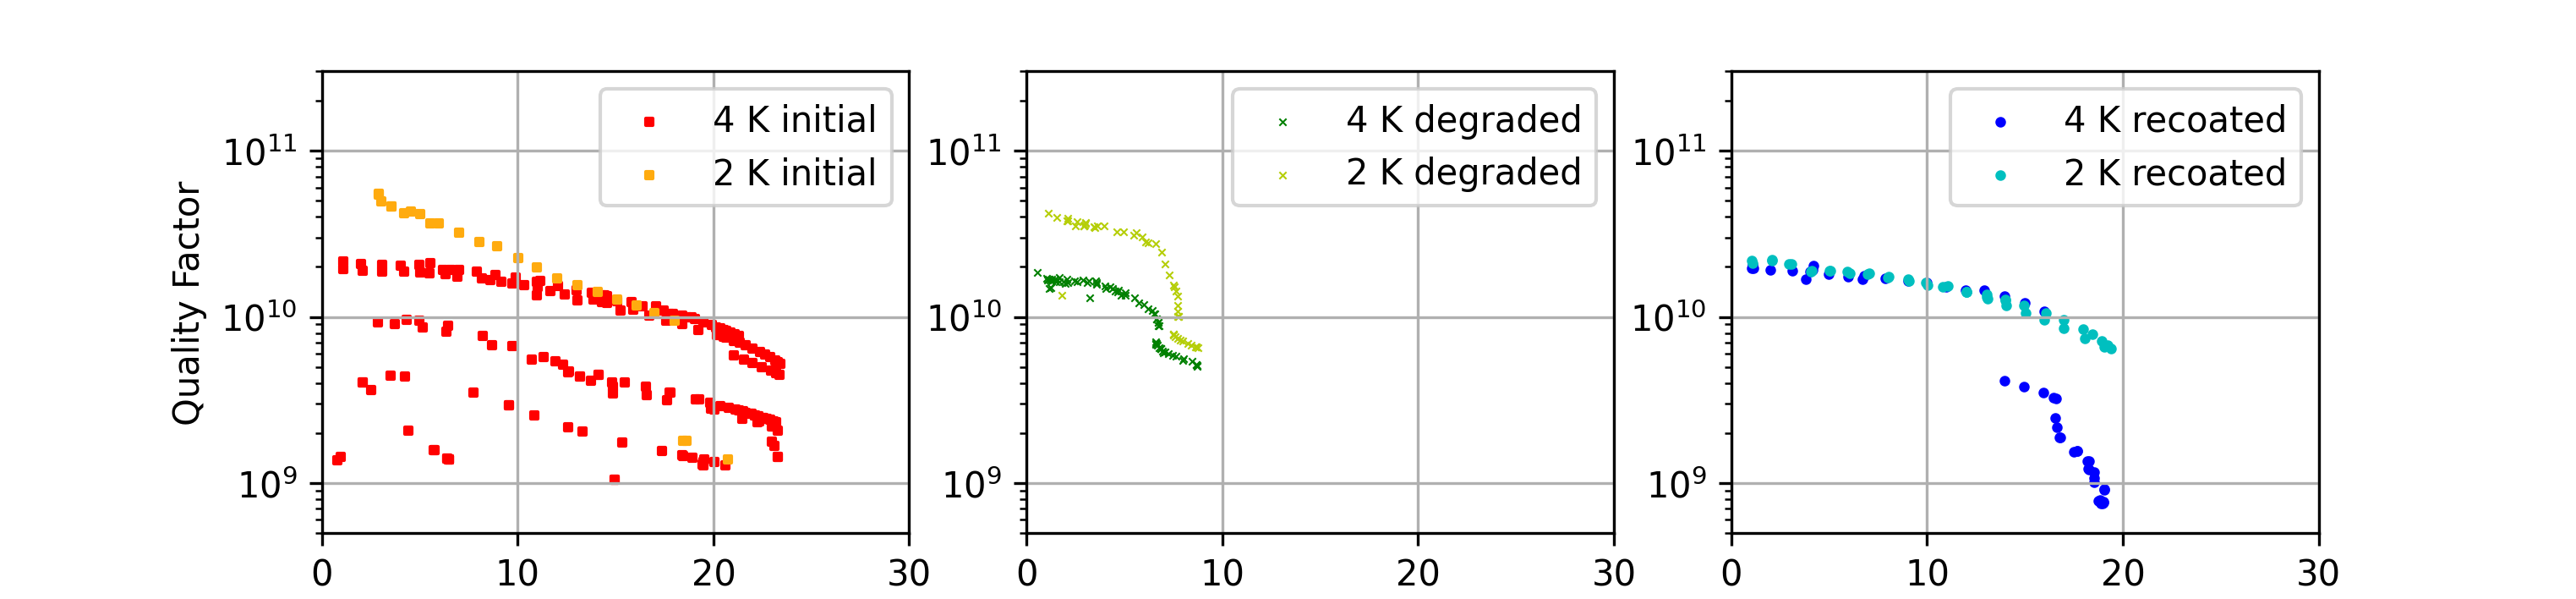
\includegraphics[width=1.0\columnwidth]{./figures/VTS.png}%
    \caption{The quality factor, indicated by dots, and X-ray emissions, indicated by x, versus the accelerating gradient of the cavity after the initial coating (A), after the degradation (B), and after the recoating (C). The quality factor and accelerating gradient where the T-maps in figure~{\protect\ref{fig:TMAP}} are measured from are shown by a red cross.}%
    \label{fig:VTS}%
\end{figure}

\begin{figure}[h]%
    \centering%
    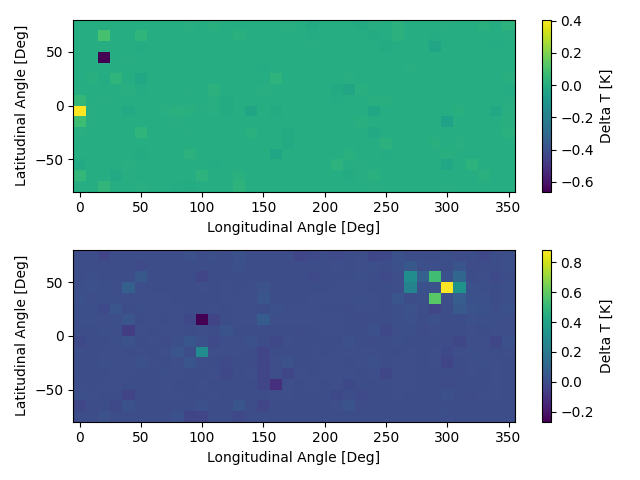
\includegraphics{./figures/TMAP.png}%
    \caption{Temperature maps of the cavity surface just before quench as measured before (top) and after (bottom) the recoating was applied. The hot spot near the equator of the recoated cavity is plotted off-scale and reached a maximum value of \qty{3}{\kelvin}}%
    \label{fig:TMAP}%
\end{figure}

After the initial coating the cavity reached a peak accelerating field of \qty{24}{\mega\volt\per\meter} and maximum Q of \num{2e10} at \qty{4}{\kelvin}. The peak accelerating gradient after the degradation was \qty{8}{\mega\volt\per\meter} and maximum Q of \num{1e10} at \qty{4}{\kelvin}. The cavity shows a decrease in quality factor around \qty{6}{\mega\volt\per\meter} before quench. A similar drop in quality factor was seen in other cavities affected by performance degradation\cite{eremeev2023preservation,eremeev:srf2019-mop015} and in Nb\textsubscript{3}Sn cavities treated with centrifugal barrel polishing\cite{viklund2024improving}. Temperature mapping as shown in figure~\ref{fig:TMAP} was used to locate the quench source responsible for the performance degradation. A single hot spot on the equator of the cavity was discovered. Visual inspection of the cavity showed no visible defects near the quench location.

After the recoating was applied the cavity performance increased. The peak accelerating gradient increased to \qty{19}{\mega\volt\per\meter} and the quality factor was \num{1e10} at \qty{4}{\kelvin}. Temperature mapping of the cavity after the recoating shows that a similar small hotspot exists close to the equator, but the hot spot is activated at higher accelerating gradients. This indicates that the source of the degradation has been at least partially repaired by the recoating. In addition to the small hot spot near the equator, there is also a much larger hot spot closer to the iris which appears just before the cavity quench. This additional hotspot is accompanied by a large increase in x-ray emissions as shown in figure~\ref{fig:VTS}, which could indicate the heating is caused by multipacting. However, higher accelerating gradients were not attainable even after \qty{5}{\hour} of processing. The cavity also did not show any signs of multipacting during the \qty{2}{\kelvin} measurement.



\section*{Discussion}
\label{sec:Discussion}

Recoating a Nb\textsubscript{3}Sn cavity that has been damaged can have a major impact on its performance. However, the mechanism for this change has not been explained. We propose two possible mechanisms for the recoating to heal the Nb\textsubscript{3}Sn film. The first mechanism is by filling in the cracks. When the cavity is exposed to Sn, a thin layer of liquid Sn is deposited on the surface which can fill up the cracks. Nb\textsubscript{3}Sn is then formed in the cracks by the diffusion of Nb into the liquid Sn. The diffusion rate of Nb is relatively slow compared to the diffusion of Sn, however if the cracks are very small, less than a few \qty{100}{nm}, the Nb may still have time to diffuse into the crack. The second mechanism to consider is the diffusion of Sn into the Nb substrate via the crack. If the crack penetrates the Nb\textsubscript{3}Sn film, Sn can diffuse into the crack and react with the Nb substrate creating a region of new Nb\textsubscript{3}Sn. This new region acts as a bridge for the electrical currents to flow through the film and prevents current flow through the Nb substrate, which has a much higher resistance than Nb\textsubscript{3}Sn. 




\section{Conclusion}
\label{sec:Conclusion}

Using a low temperature, short duration Sn recoating process, we were able to heal a degraded Nb\textsubscript{3}Sn cavity that suffered damage during transportation. The recoating improved the maximum gradient of the cavity from \qty{8}{\mega\volt\per\meter} to \qty{19}{\mega\volt\per\meter}, which is close to the initial performance of the cavity of \qty{24}{\mega\volt\per\meter}. Temperature mapping measurements of the cavity show that a single defect on the equator of the cavity was responsible for the performance degradation. After the recoating this defect was partially healed leading to less heating and a higher maximum gradient.

This discovery provides a new tool that can be applied to similarly degraded cavities to recover performance. This will save time and money that would otherwise be spent by stripping the Nb\textsubscript{3}Sn coating and applying a new coating. The process could make Nb\textsubscript{3}Sn cavities more viable for real-world accelerator applications by reducing the cost of manufacturing and transportation errors.



\bibliographystyle{plain}
\bibliography{bib}

\end{document}